\documentclass[border=6pt]{standalone}
\usepackage[T1]{fontenc}
\usepackage[utf8]{inputenc}
\usepackage[scaled=0.98]{helvet}
\renewcommand{\familydefault}{\sfdefault}
\usepackage{amsmath}
\usepackage{graphicx}
\graphicspath{{../../../../../../exercises_lecturenotes/lecture_notes/kurs100_lektionsnoter/}}
\usepackage{tikz}
\usepackage{pgfplots}
\pgfplotsset{compat=1.18}
\usetikzlibrary{arrows.meta, decorations.pathreplacing, calc, positioning, fit, backgrounds, shapes.geometric}
\usepgfplotslibrary{groupplots,fillbetween}
\definecolor{scanpink}{HTML}{E5006D}
\definecolor{scanteal}{HTML}{00A6A6}
\definecolor{scannavy}{HTML}{243746}
\definecolor{scanlightgray}{HTML}{F1F2F3}
\definecolor{ScanBlue}{RGB}{24,73,169}
\definecolor{ScanGreen}{RGB}{55,140,75}
\definecolor{ScanOrange}{RGB}{235,120,40}
\definecolor{ScanDark}{RGB}{45,45,45}
\definecolor{ScanGray}{RGB}{130,130,130}
\begin{document}
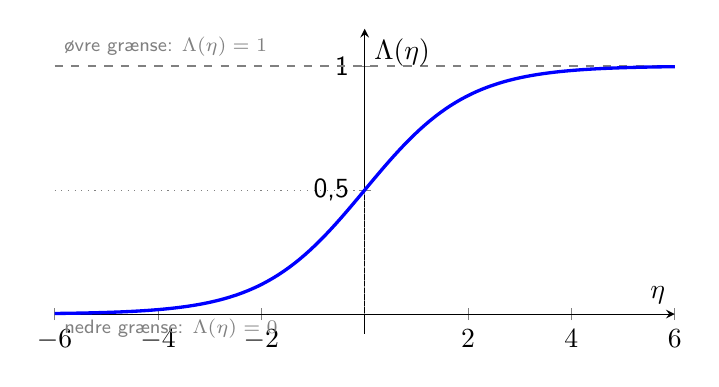
\begin{tikzpicture}
\begin{axis}[
    width=0.78\textwidth,
    height=0.45\textwidth,
    xlabel={$\eta$},
    ylabel={$\Lambda(\eta)$},
    xmin=-6, xmax=6,
    ymin=-0.08, ymax=1.15,
    axis lines=middle,
    ytick={0.5,1},
    yticklabels={{0{,}5},{1}},
    xtick={-6,-4,-2,2,4,6},
    domain=-6:6,
    samples=120,
    clip=false
]
\addplot[dashed, gray, thick] coordinates {(-6,1) (6,1)};
\addplot[dotted, gray] coordinates {(-6,0.5) (0,0.5)};
\addplot[dotted, gray] coordinates {(0,0) (0,0.5)};
\addplot[very thick, blue] {1/(1+exp(-x))};
\node[anchor=south west, font=\scriptsize, gray] at (axis cs:-6,1) {øvre grænse: \(\Lambda(\eta)=1\)};
\node[anchor=north west, font=\scriptsize, gray] at (axis cs:-6,0.02) {nedre grænse: \(\Lambda(\eta)=0\)};
\end{axis}
\end{tikzpicture}
\end{document}
